% !TeX spellcheck = en_US
\addscenariosection{1}{Clash/Alliance Scenario}{Astral Run}{\images/astral.png}

\begin{multicols*}{2}

\textbf{Author:} Laamakala

\textit{Every move could be your last. Every gate a gamble. Glory belongs to the bold.}

\subsection*{\MakeUppercase{Scenario Length}}
This Scenario plays out over 15 Rounds.

\subsection*{\MakeUppercase{Player Setup}}
\textbf{Player Count:} 2 -- 6

\textbf{Starting Resources:} 10 \svg{gold}, 2 \svg{building_materials}, 1 \svg{valuables}

\textbf{Starting Income:} 10 \svg{gold}, 0 \svg{building_materials}, 0 \svg{valuables}

\textbf{Starting Units:}

\begin{itemize}
  \item A Pack of chosen \bronze\ Units
  \item A chosen Neutral \bronze\ Unit from the player's Faction
\end{itemize}

\textbf{Town Buildings:}
\begin{itemize}
  \item \bronze\ Dwelling
\end{itemize}

\subsection*{\MakeUppercase{Map Setup}}
Take the following Map Tiles ($P$ stands for the number of players) and arrange them as shown in the Scenario map layout:

\begin{itemize}
  \item P × Starting (I) Map Tile
  \item 2P × Far (II-III) Map Tiles
  \item P × Near (IV-V) Map Tiles
  \item 6 × Near (IV-V) Map Tiles with Obelisk
  \item 1 × Center (VI-VII) Map Tile
\end{itemize}

\subsection*{\MakeUppercase{Victory Conditions}}
The game ends when any of the following conditions are met:

\begin{itemize}
  \item One player has flagged all 6 Obelisks. \textit{That player wins the game immediately.}
  \item \textbf{4 -- 6 players:} One player has defeated each of the other players' Main Heroes once. \textit{That player wins the game immediately.}
  \item At the end of Round 15.
\end{itemize}

\subsection*{\MakeUppercase{Victory Points}}
If no player has achieved an immediate victory, the player with the most Victory Points (VP) wins.

\begin{itemize}
  \item 4 VPs for the first player to flag the Center VII Field.
  \item 2 VPs for each enemy Main Hero defeated.
  \item 1 VP for each flagged Obelisk.
\end{itemize}

\subsection*{\MakeUppercase{Timed Events}}
\textbf{\nth{4} Round:}
\begin{itemize}
  \item Remove all Black Cubes from the Map, except those on Learning Stones.
\end{itemize}
\textbf{\nth{6} Round:}
\begin{itemize}
  \item Player(s) whose Main Hero has the least \svg{experience}, Search (2) \svg{artifact}.
\end{itemize}
\textbf{\nth{8} Round:}
\begin{itemize}
  \item Repeat the event of Round 4.
\end{itemize}
\textbf{\nth{10} Round:}
\begin{itemize}
  \item Player(s) whose Main Hero has the least \svg{experience}, gain 2 \svg{resource}.
\end{itemize}
\textbf{\nth{12} Round:}
\begin{itemize}
  \item Repeat the event of Round 4.
\end{itemize}

\subsection*{\MakeUppercase{Additional Rules}}
\begin{itemize}
  \item The Blocked Field on the Map Tile in the center is not considered blocked.
  \item \textbf{Sanctuary:} Search (2) your Deck. \textit{Visitable once per Faction}.
  \item \textbf{Obelisk:} Guarded by Level VI Neutral Units. Search (2) \svg{skill}, \svg{spellpower} or \svg{artifact}. \textit{Can be flagged by all players.}
  \item Each \textbf{blocked Field} adjacent to an Obelisk is a two-way Astral Gate, which only becomes active after that Obelisk has been visited.
  \item \textbf{Astral Gate:} Cannot be entered from a different Map Tile. When a Hero enters an Astral Gate, they are teleported to the Astral Gate on the Near Tile directly opposite the Center Tile. If that Tile is undiscovered, that player immediately discovers it.
  \item Gain 1 \svg{experience} after a Combat against an enemy Main Hero, unless one of the players Surrenders or Retreats.
\end{itemize}

\vspace*{\fill}
\begin{center}
  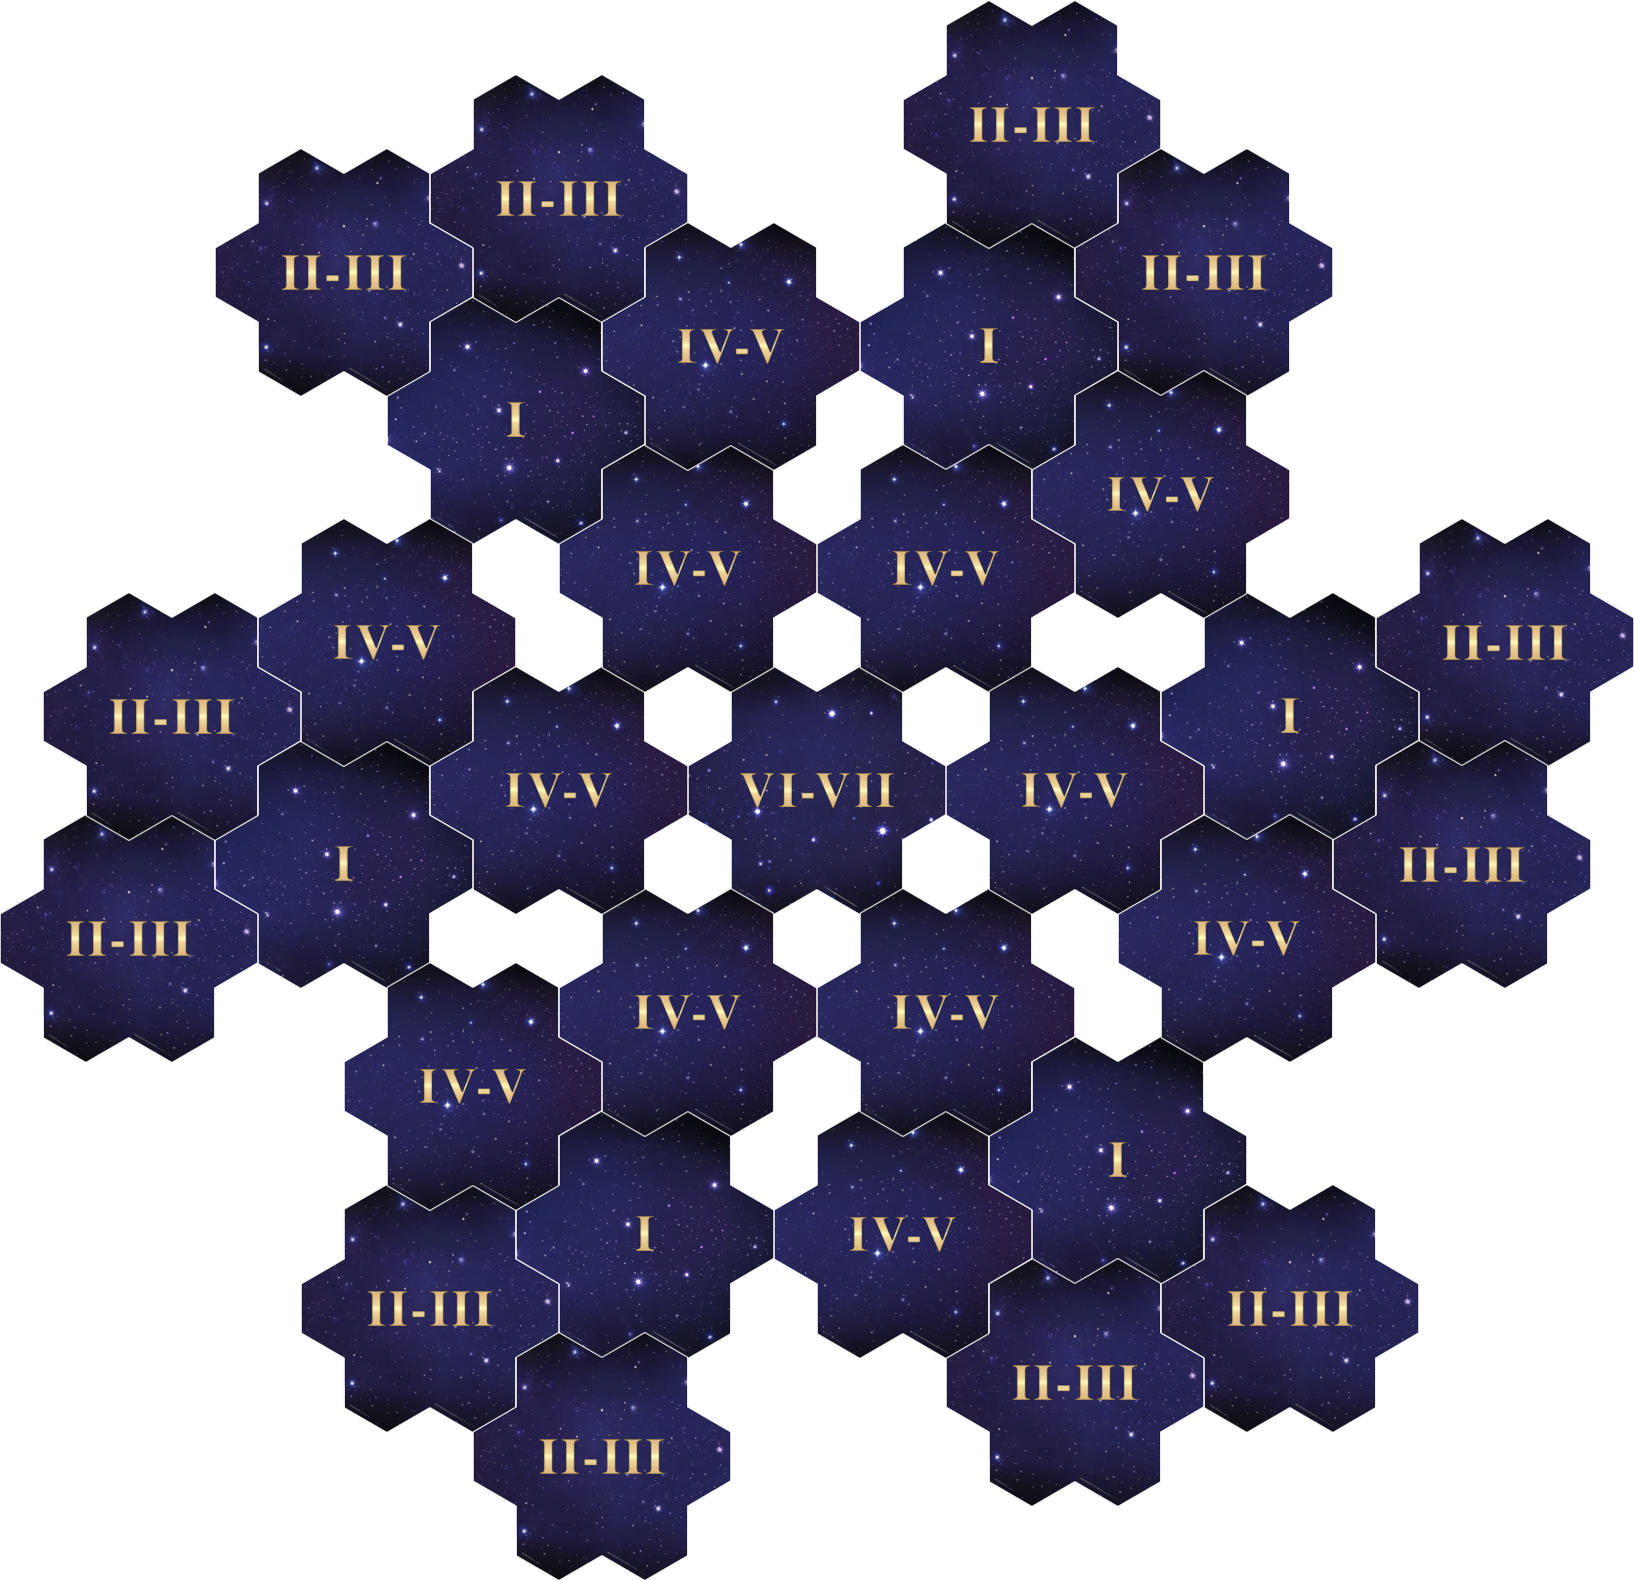
\includegraphics[width=1.16\linewidth]{\maps/astral_run.png}
  \captionof{figure}{\textbf{SCENARIO MAP LAYOUT}}
\end{center}

\columnbreak

\begin{itemize}
  \item A defeated Main Hero may Empower one Defense Statistic Card from their M\&M Deck.
  \item \textbf{Level VII Settlement:} Increase all incomes by 1 space.
  \item \textbf{Random Town:} You may recruit one Faction Unit you defeated for half its recruitment cost or increase all incomes by one space.
  \item \textbf{Dragon Utopia:} Take any Card from your Discard pile. You may recruit one dragon you defeated for half its recruitment cost.
  \item \textbf{11-Round game:} Remove P × Near (IV-V) Map Tiles and replace the Center (VI-VII) Tile with a Near (IV-V) Map Tile without an Obelisk.
\end{itemize}

\begin{center}
  \hspace*{-2em}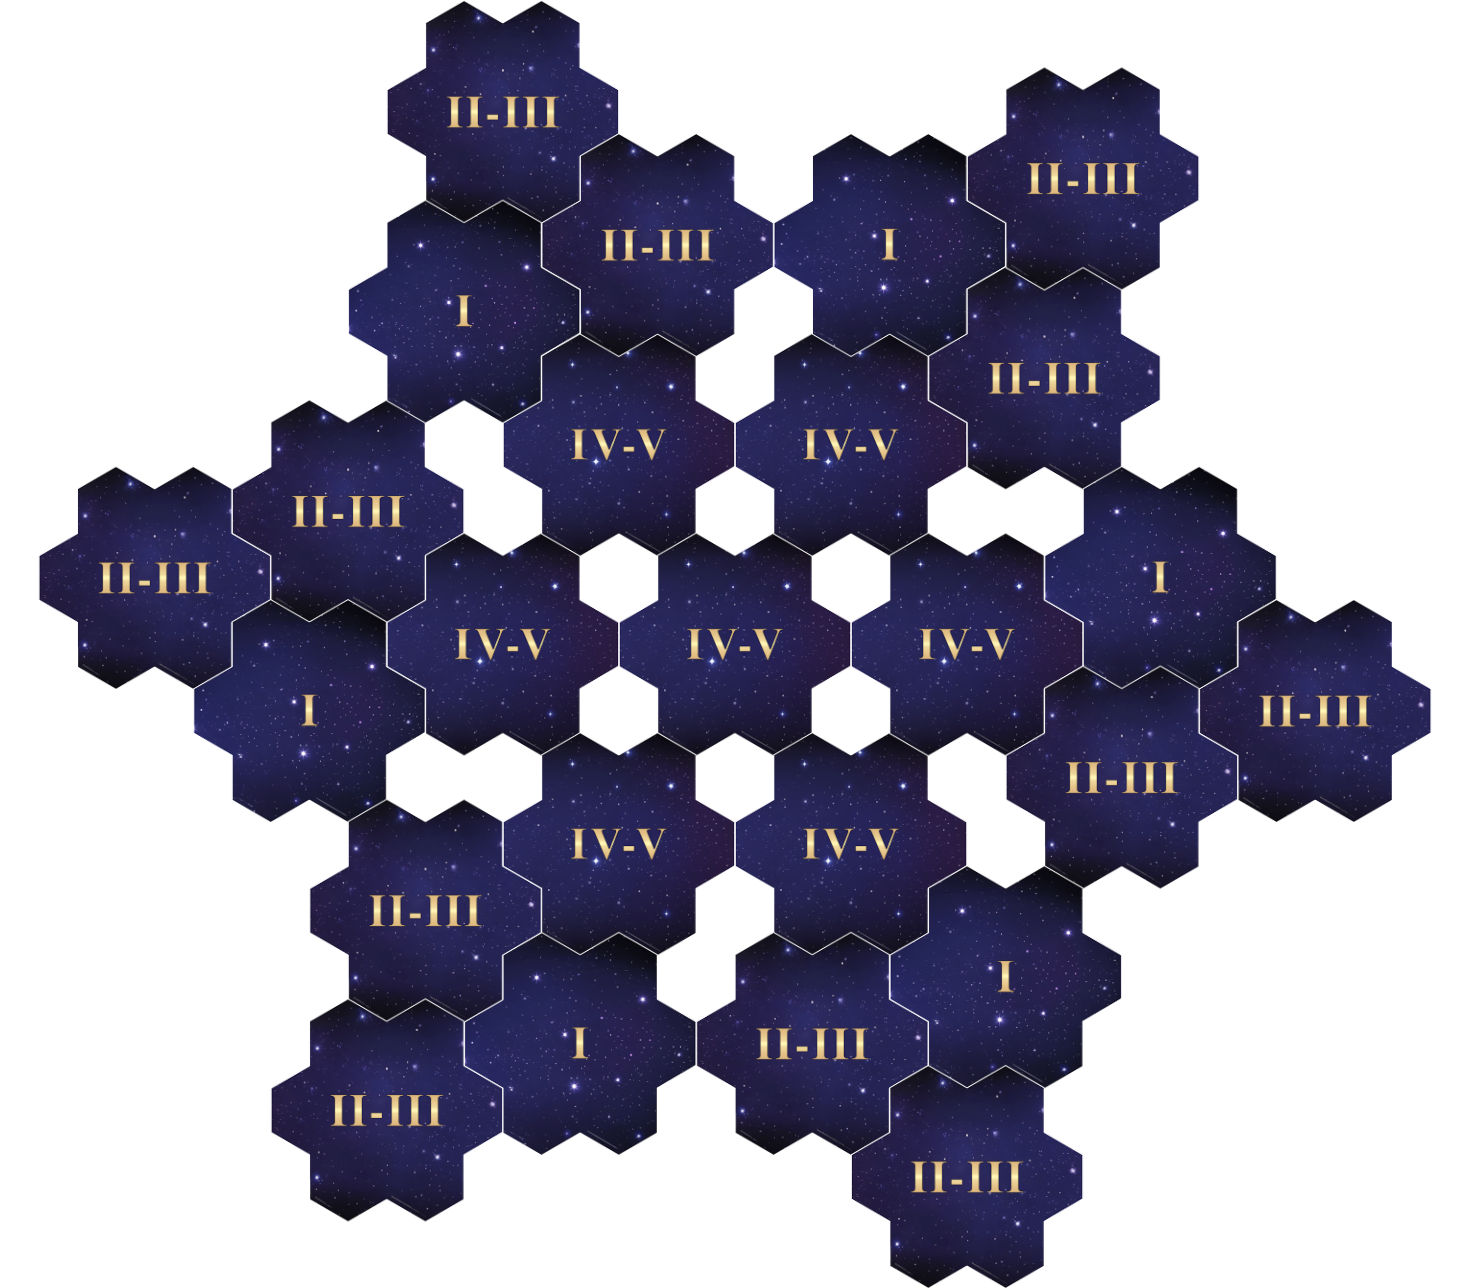
\includegraphics[width=1.16\linewidth]{\maps/astral_run_short.png}
  \vspace*{-1em}
  \hspace*{2em}\captionof{figure}{\textbf{SHORT GAME MAP LAYOUT}}
\end{center}
\vspace*{\fill}

\end{multicols*}
